\chapter{实验}
第三章针对流式数据的特点,提出了一种利用网格的改进的增量LOF快速异常数据检测算法,不但可以减少存储空间,也可以减少计算量,加快检测速度。第四章针对流式数据中时序数据的特点,分别对周期时间采样的时序数据和非周期时间采样的时序数据提出加速的计算方式,分别建立缓存和使用增量计算,减少矩阵的计算次数,实现快速压缩。为了验证所提算法的有效性,本章设计了多组对照实验,进行了多方面的性能比较。

\section{实验环境}
所有的实验的运行环境为Windows 7,64位操作系统,CPU为3.40GHz,安装内存为8.00GB。使用Java语言在Eclipse上编程实现,并且用Python实现结果的可视化。

\section{异常数据检测对比实验}
在本节内容中,进行异常数据检测的对比实验。测试实验采用的数据集一共有两种,一种是真实数据集KDD CUP-99\upcite{KDDData},这个数据集是由MIT林肯实验室收集的网络入侵检测数据集。另外,为了可以更好地将算法运行的结果可视化,另一种测试的数据集是人工数据集,称其为RandomSet。

\subsection{人工数据集的对比实验}
人工数据集RandomSet共有$11,000$条数据记录,是一个二维数据集,每一维数据类型都为实数,第一维数据的范围在$0\sim 520$,第二维数据范围为$0\sim 260$。RandomSet的分布如图\ref{fig:fig51}所示,数据共可以聚为4类,其中两类数据,分布比较均匀,但是数据量较少,分布比较稀疏。另外两类,中心密度较高,周围数据点分布比较松散。在整个数据集中,有些游离在类外的数据点。该数据集主要用来进行增量的LOF算法与本算法的对比实验,包括异常点检测的精确度对比,运行时间对比和运行内存对比。

\begin{figure}[htb]
	\centering
	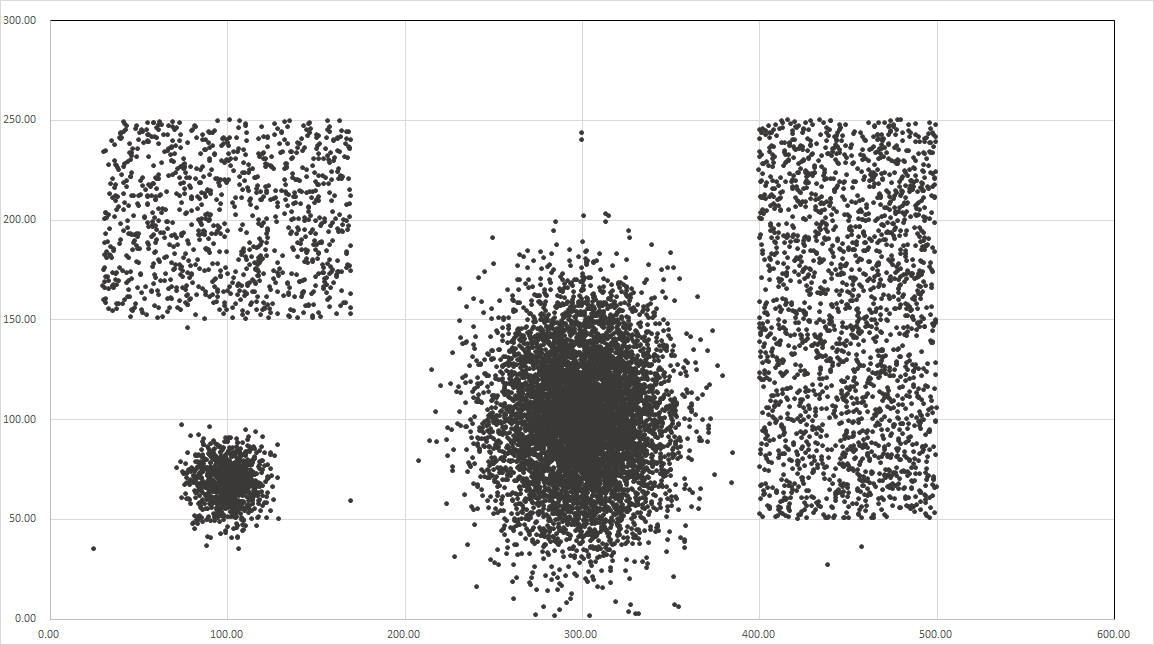
\includegraphics[width=0.55\textwidth]{figures/figure5x1}
	\caption{人工数据集RandomSet}\label{fig:fig51}
\end{figure}

数据集RandomSet是随机生成的,由图\ref{fig:fig51}可以看出,虽然四个类的密度不同,但是根据异常数据的定义,异常数据点主要是在类外面的游离的数据点和分布在圆形数据类的外侧边缘的数据点。在实验中,各类的数据点以及异常数据点交替出现,特别是异常数据点,随机地出现在数据流中,次序是随机的。在实验中,$k$取值为180。每个维度平均分段,段的长度$len$取值为5。则本算法的异常数据检测的结果与增量的LOF算法的结果如图\ref{fig:fig534}所示。其中$X_1$表示第一维,$X_2$代表第二维,$LOF$代表检测出来的因子。$LOF$越大,是异常值的可能性就越大。

\begin{figure}[htbp]
	\centering                                      %居中
	\subfigure[改进的增量LOF快速检测算法]{              %第一张子图
		\begin{minipage}{7cm}
			\label{fig:fig53}
			\centering                              %子图居中
			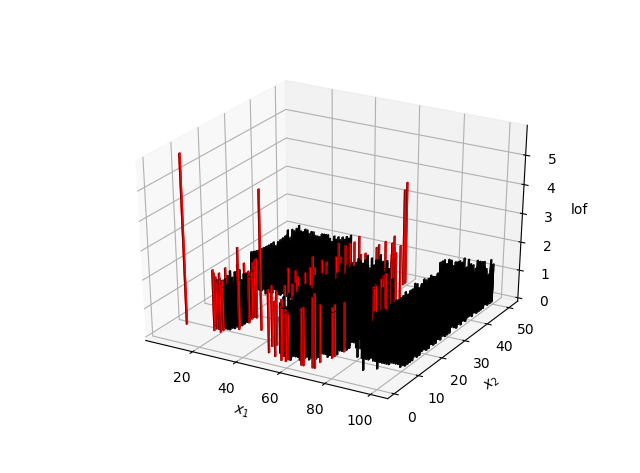
\includegraphics[width=0.99\textwidth]{figures/figure5x3}   %以pic.jpg的0.5倍大小输出
		\end{minipage}
	}
	\subfigure[增量LOF算法]{                  %第二张子图
		\begin{minipage}{7cm}
			\label{fig:fig54}
			\centering                                  %子图居中
			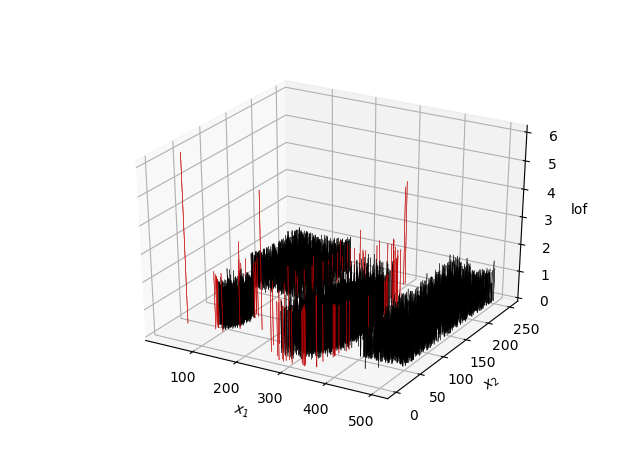
\includegraphics[width=0.99\textwidth]{figures/figure5x4}       %以pic.jpg的0.5倍大小输出
		\end{minipage}
	}\caption{在RandomSet上两种方法的异常数据检测结果} %                     %大图名称
	\label{fig:fig534}                                       %图片引用标记
\end{figure}

其中,图\ref{fig:fig53}是本文提出的算法的检测结果,图\ref{fig:fig54}是增量的LOF算法的检测结果。由两图对比可知,本算法检测出来的异常网格与增量的LOF算法检测出来的异常数据的局部异常因子基本一致,也符合图\ref{fig:fig51}的直观感受到的异常数据。

为了验证本文提出算法的加速效果,选择了连续的$2000$个数据点,记录每个数据点到来后进行检测的时间,其结果如图\ref{fig:fig55}所示。
\begin{figure}[htbp]
	\centering                                      %居中
	\subfigure[改进的增量LOF快速检测算法]{              %第一张子图
		\begin{minipage}{7cm}
			\label{fig:fig551}
			\centering                              %子图居中
			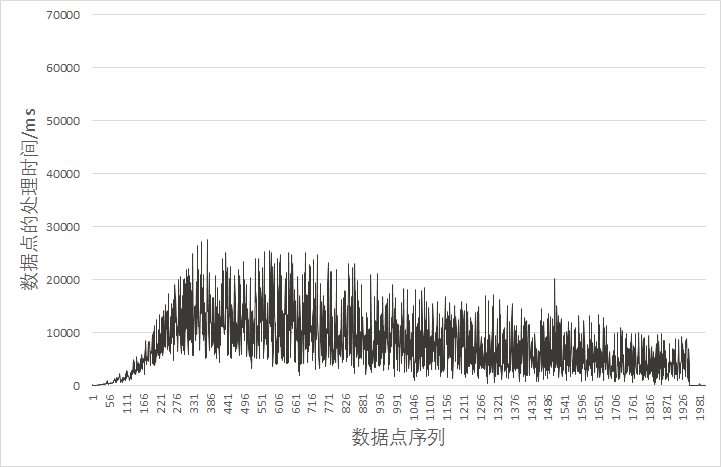
\includegraphics[width=0.9\textwidth]{figures/figure5x51}   %以pic.jpg的0.5倍大小输出
		\end{minipage}
	}
	\subfigure[增量LOF算法]{                  %第二张子图
		\begin{minipage}{7cm}
			\label{fig:fig552}
			\centering                                  %子图居中
			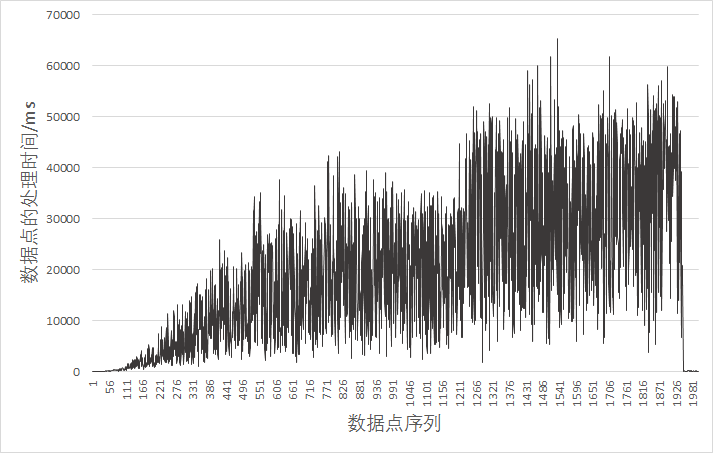
\includegraphics[width=0.9\textwidth]{figures/figure5x52}       %以pic.jpg的0.5倍大小输出
		\end{minipage}
	}\caption{在RandomSet上两种方法的运行时间对比} %                     %大图名称
	\label{fig:fig55}                                       %图片引用标记
\end{figure}
由\ref{fig:fig55}的结果可知,当数据量较少时,两种算法的运行时间基本相同,但随着数据量的增长,增量LOF算法的对每个数据点的检测时间大致在增长,而本算法对每个数据点的检测时间基本不变,并且小于增量LOF算法,所以当数据量越来越多时,本算法对每个数据点的检测时间更短,速度更快。实验的运行时内存对比如图\ref{fig:fig567}所示。在实验中,两种算法的实现程序在Eclipse中运行,运行的JVM内存参数设置为“$-Xmx4096m\  -Xms1024m$”,使用工具JConsole来查看运行时内存变化,其结果如图\ref{fig:fig567}所示,从图中可以看出,本算法的运行过程中,大部分时间的内存使用量在400MB以下,而增量的LOF算法的运行中,内存的使用量可达到1.3GB,大部分可达1.0GB以上。所以,本算法的运行过程中,内存使用量更少。

\begin{figure}[htbp]
	\centering                                      %居中
	\subfigure[改进的增量LOF快速检测算法]{              %第一张子图
		\begin{minipage}{7cm}
			\label{fig:fig56}
			\centering                              %子图居中
			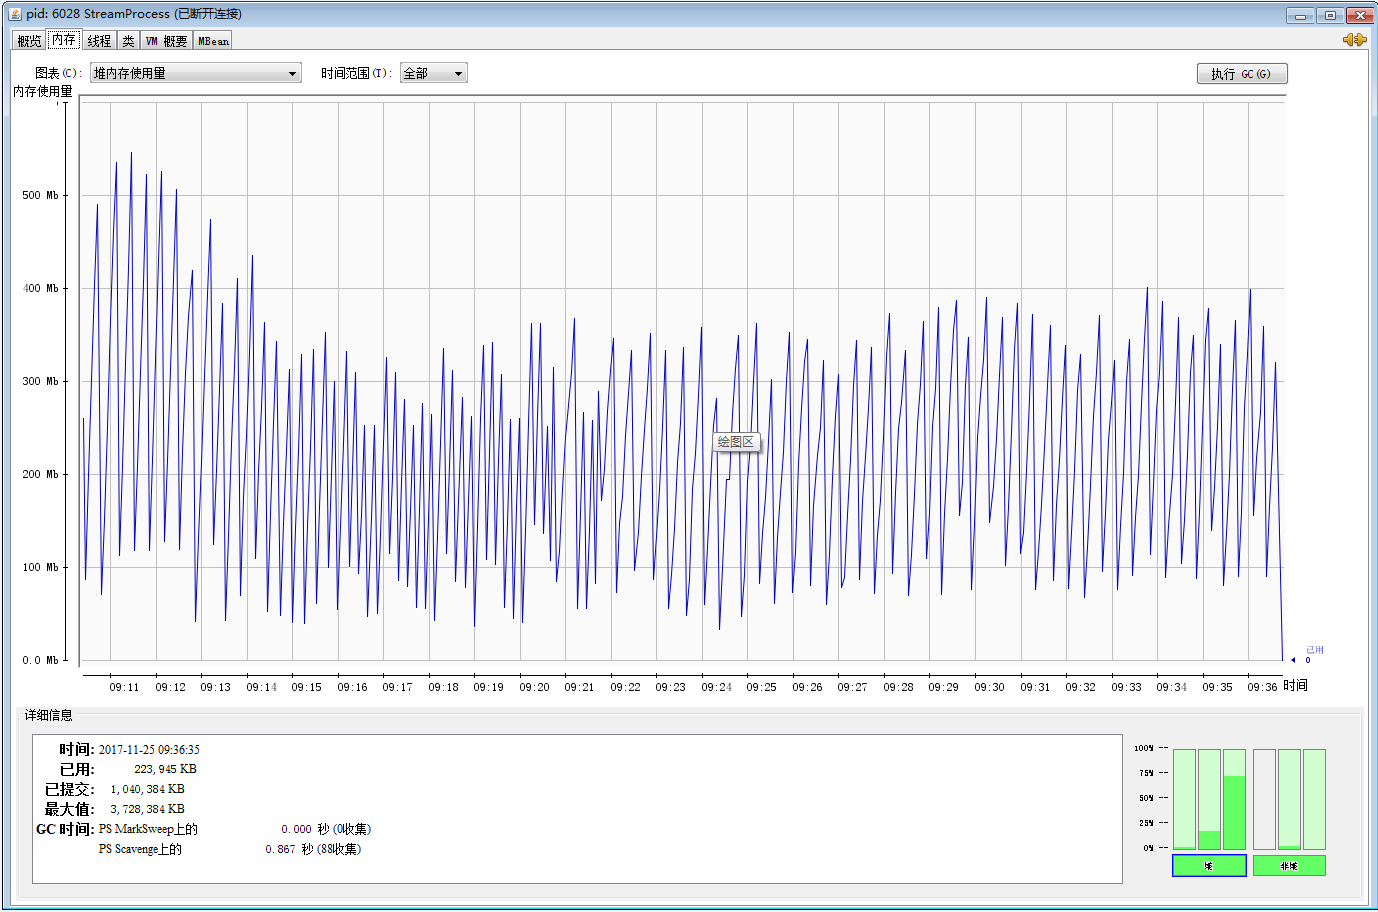
\includegraphics[width=0.9\textwidth]{figures/figure5x6}   %以pic.jpg的0.5倍大小输出
		\end{minipage}
	}
	\subfigure[增量LOF算法]{                  %第二张子图
		\begin{minipage}{7cm}
			\label{fig:fig57}
			\centering                                  %子图居中
			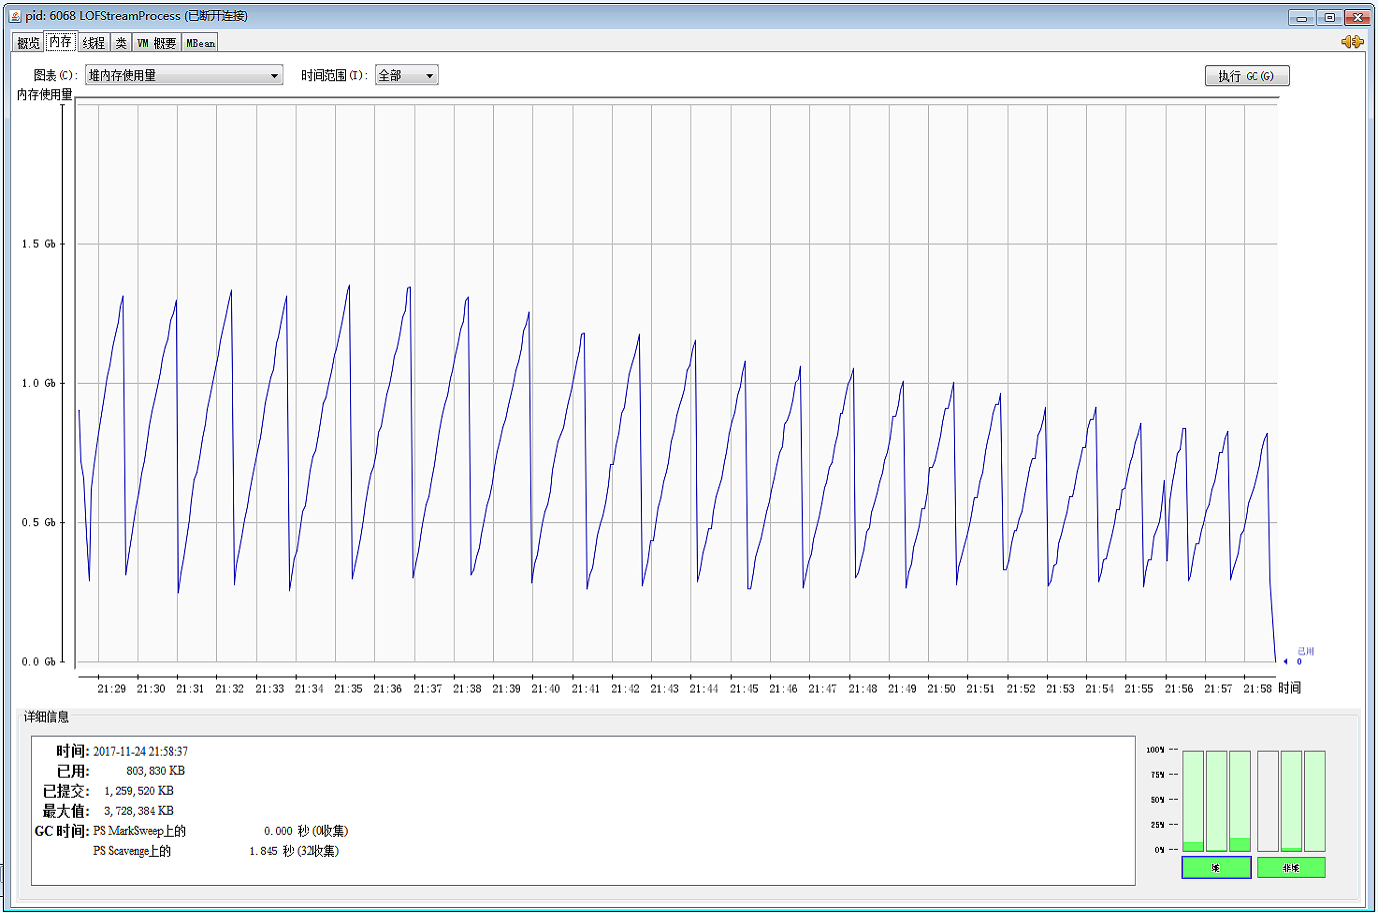
\includegraphics[width=0.9\textwidth]{figures/figure5x7}       %以pic.jpg的0.5倍大小输出
		\end{minipage}
	}\caption{在RandomSet上两种方法的运行内存变化} %                     %大图名称
	\label{fig:fig567}                                       %图片引用标记
\end{figure}

\subsection{KDD CUP-99数据集的对比实验}
KDD CUP-99数据集共有41个属性,其中,有34个属性为连续属性,有7个为离散属性,在实验中,采用34个连续的属性,并且,为了数据处理的准确性,防止属性值很大的维度占据主要的比重而忽略属性值小的维度,对数据集的各个维度做0-1标准化处理,转换函数如下:
\begin{equation}
x^{'}=\frac{x-min}{max- min}
\end{equation}
处理后的各个维度的值均在$\left [ 0,1 \right ]$之间。在实验中,各个维度的划分长度为0.05,$k$的取值为180。该实验的实验数据集是真实数据,主要进行性能测试的比较,一共选取了连续的10,000条记录来进行实验,并在其中,选择了连续的7,000条数据记录,记录了每条数据的处理时间,对比结果如图\ref{fig:fig512}所示。
\begin{figure}[htbp]
	\centering                                      %居中
	\subfigure[改进的增量LOF快速检测算法]{              %第一张子图
		\begin{minipage}{7cm}
			\label{fig:fig5111}
			\centering                              %子图居中
			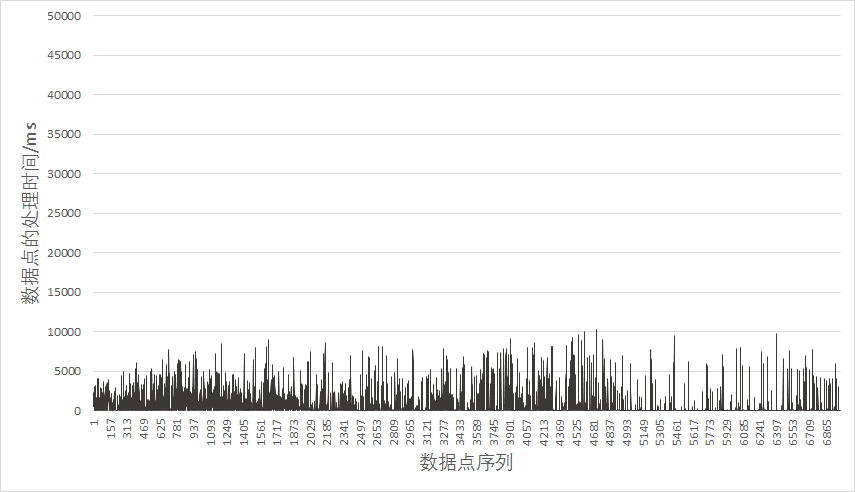
\includegraphics[width=0.9\textwidth]{figures/figure5x111}   %以pic.jpg的0.5倍大小输出
		\end{minipage}
	}
	\subfigure[增量LOF算法]{                  %第二张子图
		\begin{minipage}{7cm}
			\label{fig:fig5112}
			\centering                                  %子图居中
			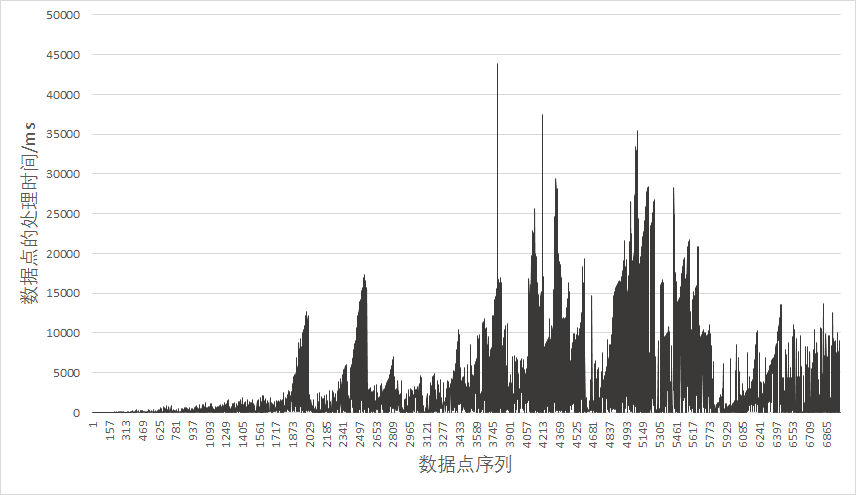
\includegraphics[width=0.9\textwidth]{figures/figure5x112}       %以pic.jpg的0.5倍大小输出
		\end{minipage}
	}\caption{在KDD CUP-99数据集上两种方法的异常数据检测结果} %    %大图名称
	\label{fig:fig512}                                       %图片引用标记
\end{figure}

从图\ref{fig:fig512}中可以看出,在开始的一段时间内,原来的增量LOF算法运行速度要更快,但是一段时间后,随着数据量的增加,本文提出的改进的增量LOF快速检测算法的处理速度更快,时间更少。而且从全局时间来看,本文提出的改进的增量LOF快速检测算法的对每个数据的处理时间维持在一个较为稳定的水平,时间波动不大,而原增量LOF算法的运行之间呈现增长趋势,这也与本文前面的分析保持一致。两种算法的程序也在Eclipse中运行,运行的JVM内存参数设置为“$-Xmx4096m\ -Xms1024m$”,使用工具JConsole来查看运行时内存变化,其结果如图\ref{fig:fig51015}所示。
\begin{figure}[htbp]
	\centering                                      %居中
	\subfigure[改进的增量LOF快速检测算法]{              %第一张子图
		\begin{minipage}{7cm}
			\label{fig:fig515}
			\centering                              %子图居中
			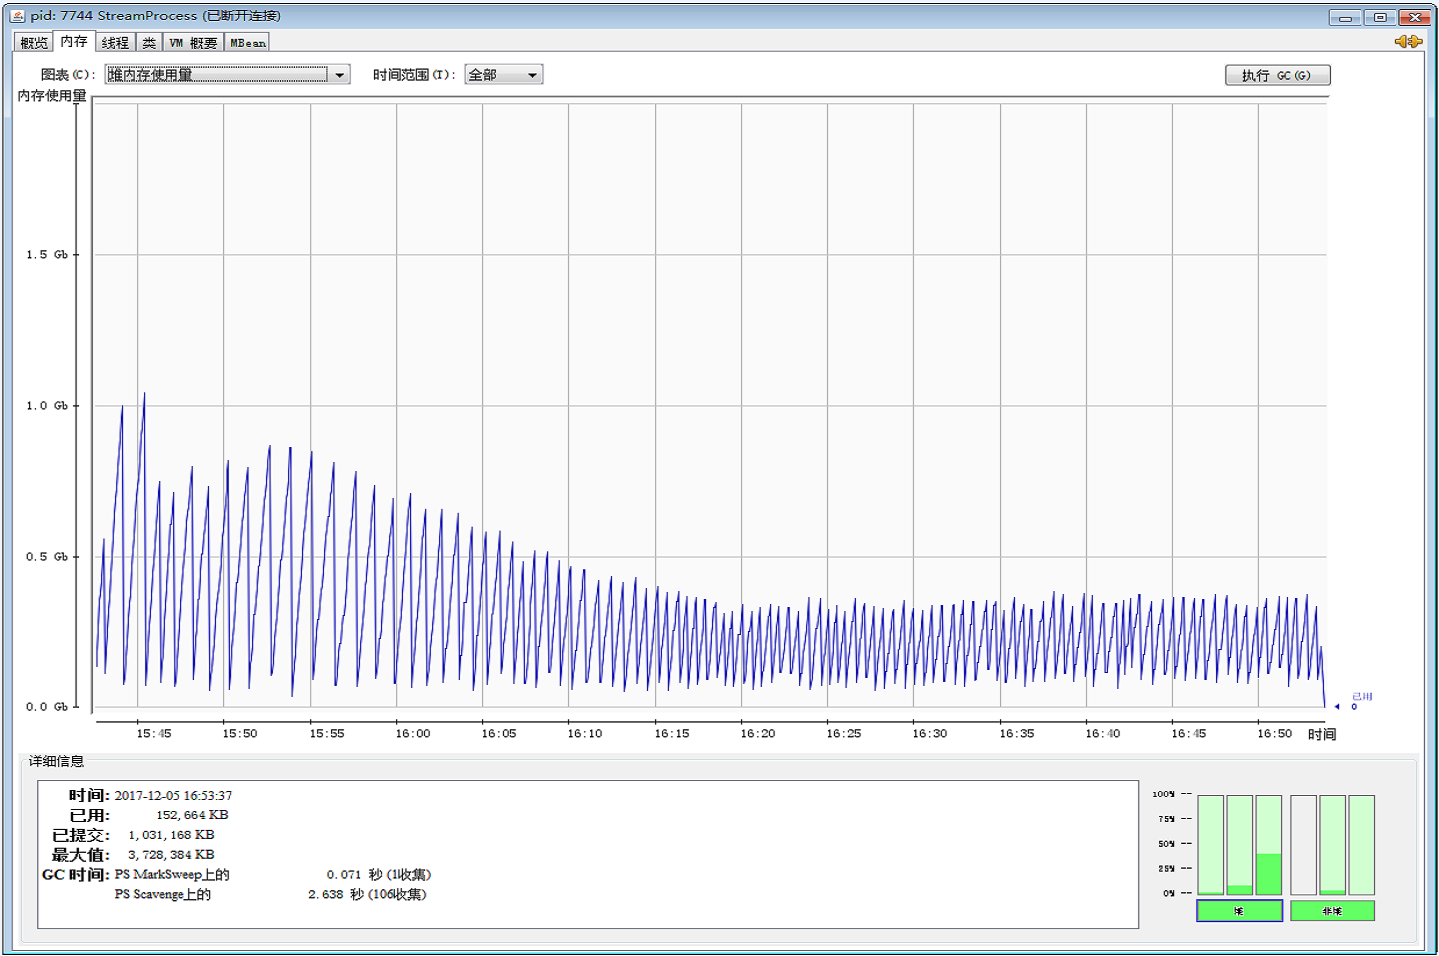
\includegraphics[width=0.9\textwidth]{figures/figure5x15}   %以pic.jpg的0.5倍大小输出
		\end{minipage}
	}
	\subfigure[增量LOF算法]{                  %第二张子图
		\begin{minipage}{7cm}
			\label{fig:fig510}
			\centering                                  %子图居中
			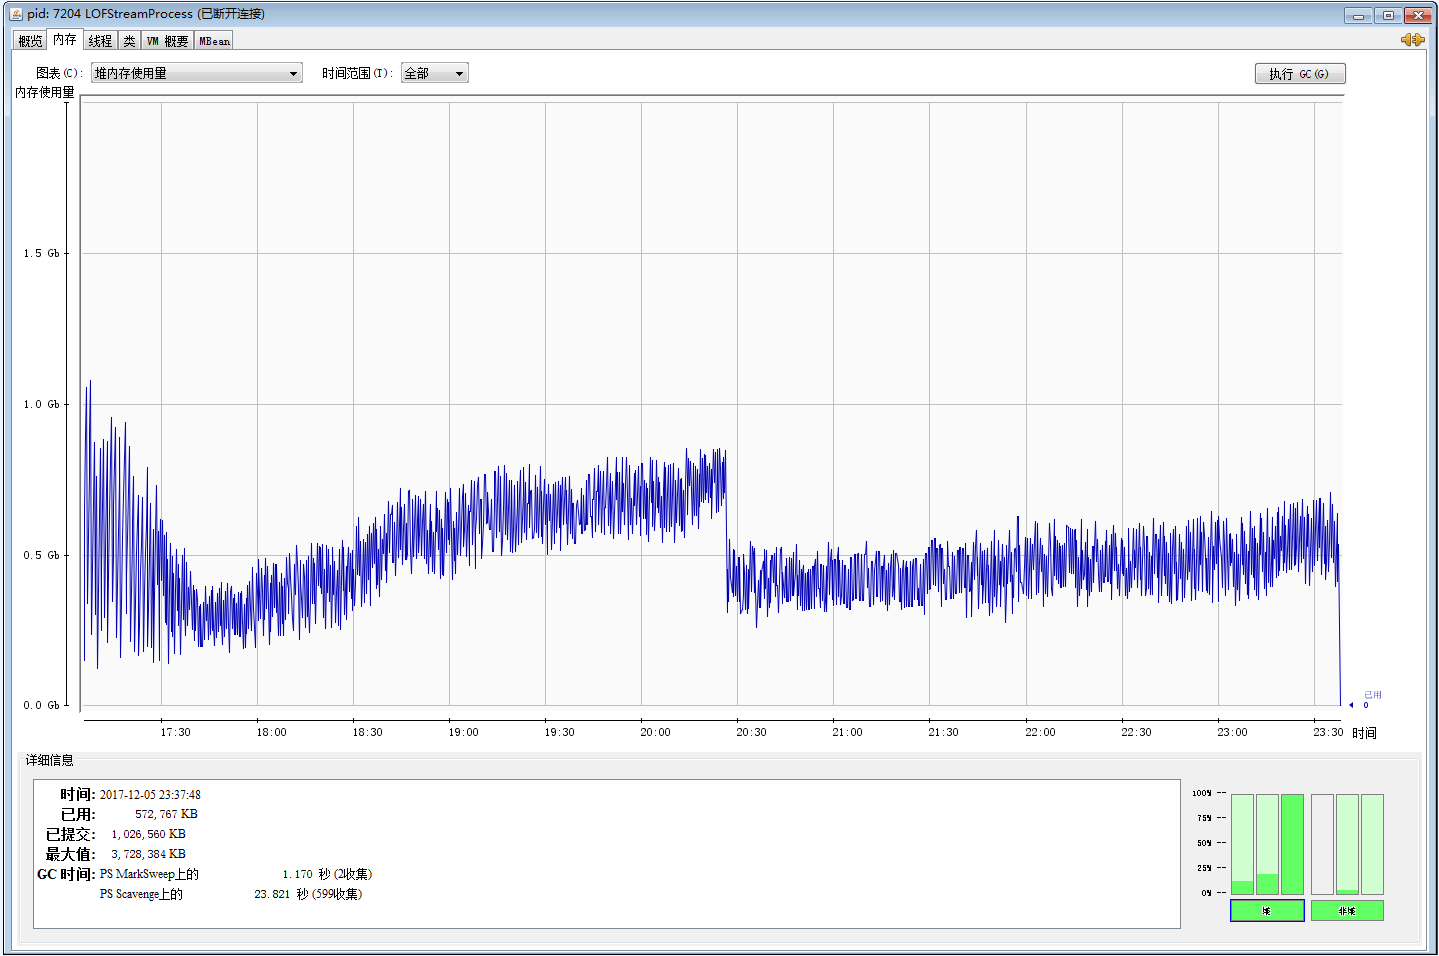
\includegraphics[width=0.9\textwidth]{figures/figure5x10}       %以pic.jpg的0.5倍大小输出
		\end{minipage}
	}\caption{在KDD CUP-99数据集上两种方法的运行内存变化} %                     %大图名称
	\label{fig:fig51015}                                       %图片引用标记
\end{figure}
在图\ref{fig:fig510}和\ref{fig:fig515}中,横坐标为运行的时间,纵坐标为内存的使用量。从图中可以看出,增量的LOF算法的运行时间长于本文提出的改进算法,在运行前期,两种算法的内存使用量基本一致,但是随着时间的增长,数据量越来越多,本文提出的算法的内存使用量保持在0.5MB以下,呈现稳定的状态,而增量的LOF算法的内存使用量越来越高,并且明显高于0.5MB。所以从对于KDD CUP-99数据集的实验中可以看出,在流式数据环境中,当数据量越来越多的时候,本算法的运行时间更少,且在运行过程中,内存使用量更少。


\section{压缩算法对比实验}
在本节内容中,进行流式时序数据的多项式压缩的对比实验。通过以下几组对比实验,来验证本文在上一章提出的加速方法的效果,是否可以很好地提高计算速度,有效地减少多项式拟合时间。实验采用三个时序数据集,其中两个数据集是周期时间采样的数据集,包括某实际生产数据集,从UCI数据库中下载得到的气体数据集\upcite{gasdata}。剩余一个是非周期时间采样的数据集,从UCI数据库中下载,是测量人体移动的传感器数据集\upcite{GaitData}。本节实验将用这些时序数据集模拟流式时序数据。

实验分别验证周期时间采样的时序数据与非周期时间采样的时序数据的加速方法的加速效果,在实验中,定义加速比为原计算方法的运行时间与加速方法的运行时间的比值。为了得到较为精确的对比,分别选取不同的拟合误差($\varepsilon $)与不同的多项式次数($k$)来进行实验对比。

\subsection{周期时间采集的流式时序数据对比实验}
周期时间采集的时序数据包括实际生产数据集和从UCI数据库中下载的气体数据集\upcite{gasdata},其中,实际生产数据集包含$5,013,811$条数据记录,UCI气体数据包含$4,178,504$条数据记录。

当测试数据集是实际生产数据集,多项式的次数$k$依次为$5,6,7,8$,并且拟合误差$\varepsilon$分别为$100,125,...,250$时,其运行结果如图\ref{fig:fig621}所示。

\begin{figure}[htb]
	\centering
	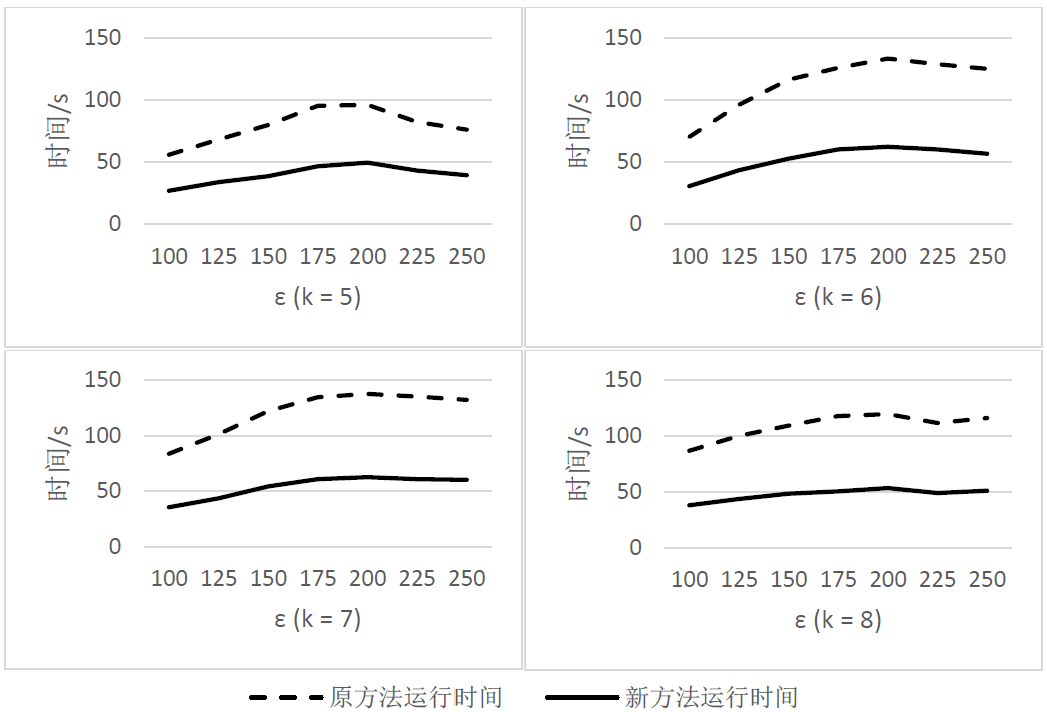
\includegraphics[width=0.55\textwidth]{figures/figure62x1product}
	\caption{周期时间采样的生产数据上的运行时间,其中$k$是多项式次数,$\varepsilon$是拟合误差}\label{fig:fig621}
\end{figure}

由图中可知,当拟合多项式次数$k$越大时,两种方法的运行时间越长。而且,当$k$不变时,随着拟合误差$\varepsilon$的增大,运行时间先变大,之后基本保持不变,这是因为拟合误差越大,每个分段后的数据段长度越长,所以每段的拟合时间会变长,但是因为因为数据量总量不变,所以段长变长后,段数会变少,所以,全体数据的拟合时间基本不变。在生产数据集上多项式拟合的加速比如图\ref{fig:fig622}所示。

\begin{figure}[htb]
	\centering
	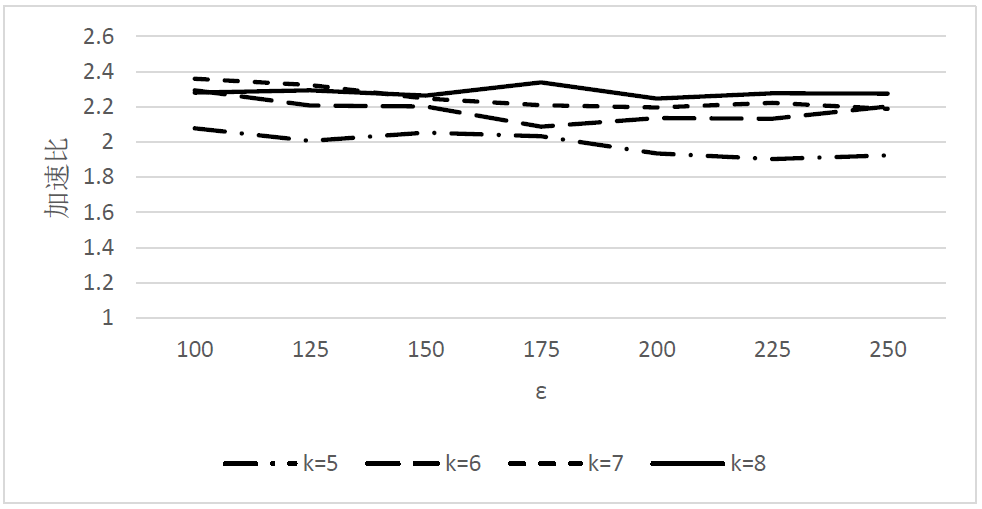
\includegraphics[width=0.55\textwidth]{figures/figure62x2product}
	\caption{周期时间采样的生产数据上的加速比,其中$k$是多项式次数,$\varepsilon$是拟合误差}\label{fig:fig622}
\end{figure}

由图\ref{fig:fig622}可知,本文提出的加速方法与原计算方法相比,具有较好的加速效果,加速比最大可达$2.4$x,而且整体来看,多项式次数$k$越大,加速效果越好。关于UCI气体数据集,将多项式次数$k$设置为$5,6,7,8$,因为其数据属性原因,所以将其拟合误差$\varepsilon$设为$5,6,7,..,10$,则运行时间结果如图\ref{fig:fig623}所示,加速比如图\ref{fig:fig624}所示。

\begin{figure}[htb]
	\centering
	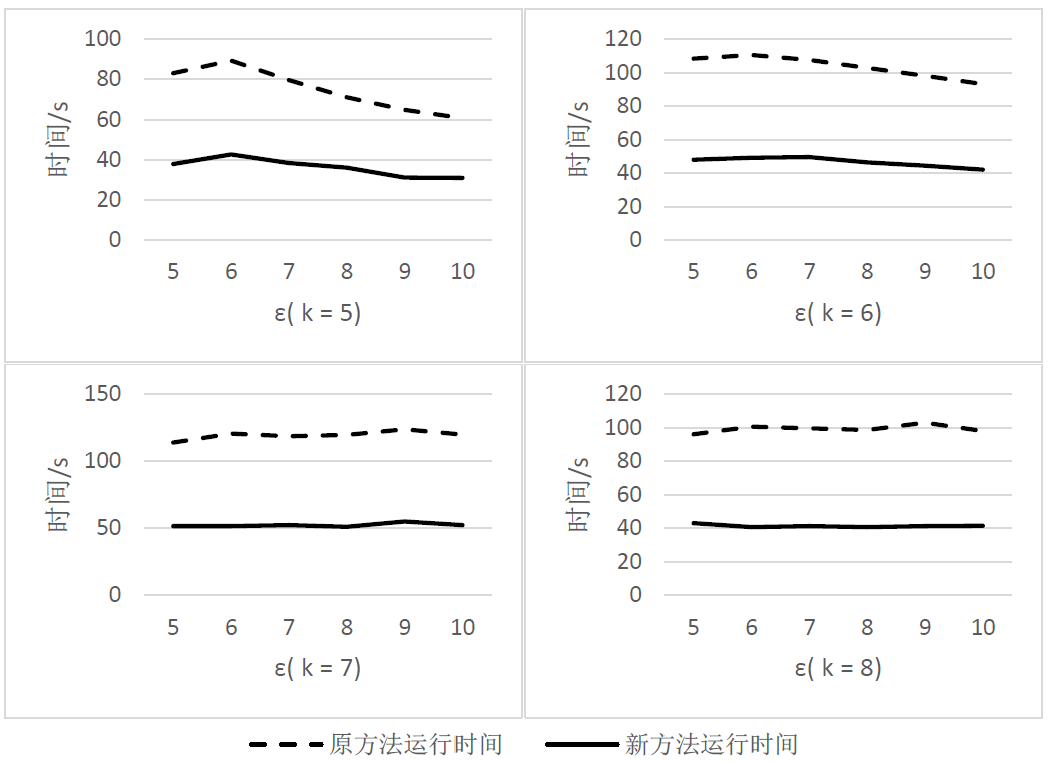
\includegraphics[width=0.55\textwidth]{figures/figure62x3gas}
	\caption{周期时间采样的UCI气体数据上的运行时间,其中$k$是多项式次数,$\varepsilon$是拟合误差}\label{fig:fig623}
\end{figure}

\begin{figure}[htb]
	\centering
	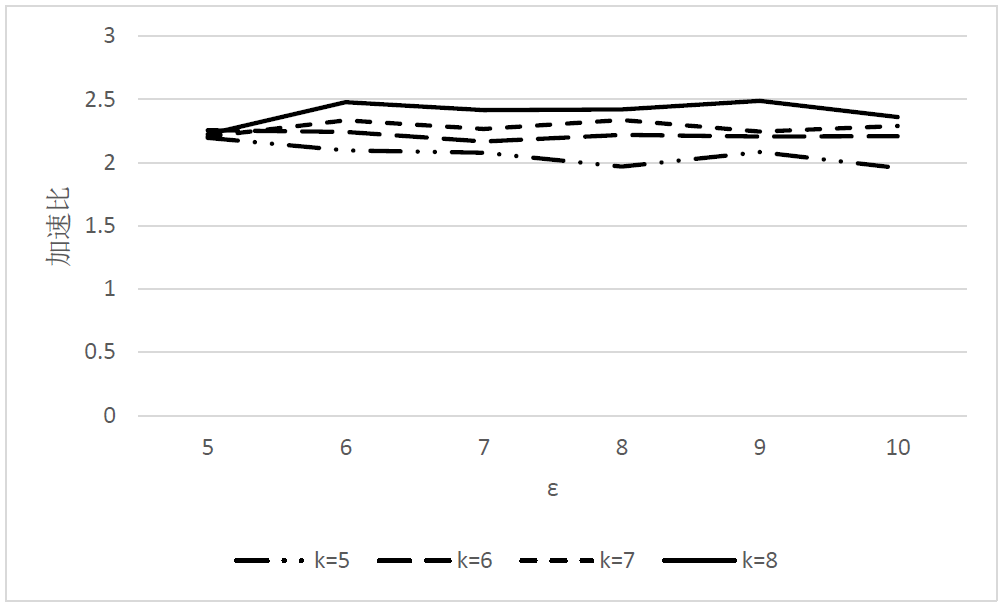
\includegraphics[width=0.55\textwidth]{figures/figure62x4gas}
	\caption{周期时间采样的UCI气体数据上的加速比,其中$k$是多项式次数,$\varepsilon$是拟合误差}\label{fig:fig624}
\end{figure}

由图\ref{fig:fig623}可知,本文提出的加速方法的运行时间少于原方法的运行时间,当$k$和$\varepsilon$变化时,总运行时间基本不变。由图\ref{fig:fig624}可知,加速比在$2$x $\sim 2.5$x之间,而且$k$越大,加速效果越好。由上面两组实验结果可知,在流式环境中,本文提出的方法计算速度更快,具有较好的加速效果,而且对于周期性采样的流式时序数据,加速比可达到$2x$。

\subsection{非周期时间采样的流式时序数据对比实验}
在关于非周期时间采样的流式时序数据的对比实验中,采用从UCI数据库中下载的非周期时间采集的测量人体移动的传感器数据集\upcite{GaitData},这个数据集有$195,737$条数据记录。因为非周期时间采集的时序数据集较少,所以为了得到更加精确的结论,将周期时间采集的UCI气体数据集\upcite{gasdata}当做非周期时间采集的数据集,来进行此组实验。所以,本组实验的实验数据包括UCI人体移动传感器数据集和UCI气体数据集。

如图\ref{fig:fig627}所示,是在UCI气体数据集上的运行结果,由图中可知,当$k$不变时,拟合误差$\varepsilon$越大,运行时间呈大致先增大后减小的趋势。而当拟合误差$\varepsilon$不变时,$k$越大,运行时间越长。所以运行时间随着多项式次数$k$的增大而增大。而且当$k$与$\varepsilon$相同时,本文提出的加速方法,运行时间要少于原方法。其加速比如图\ref{fig:fig628}所示。

\begin{figure}[htb]
	\centering
	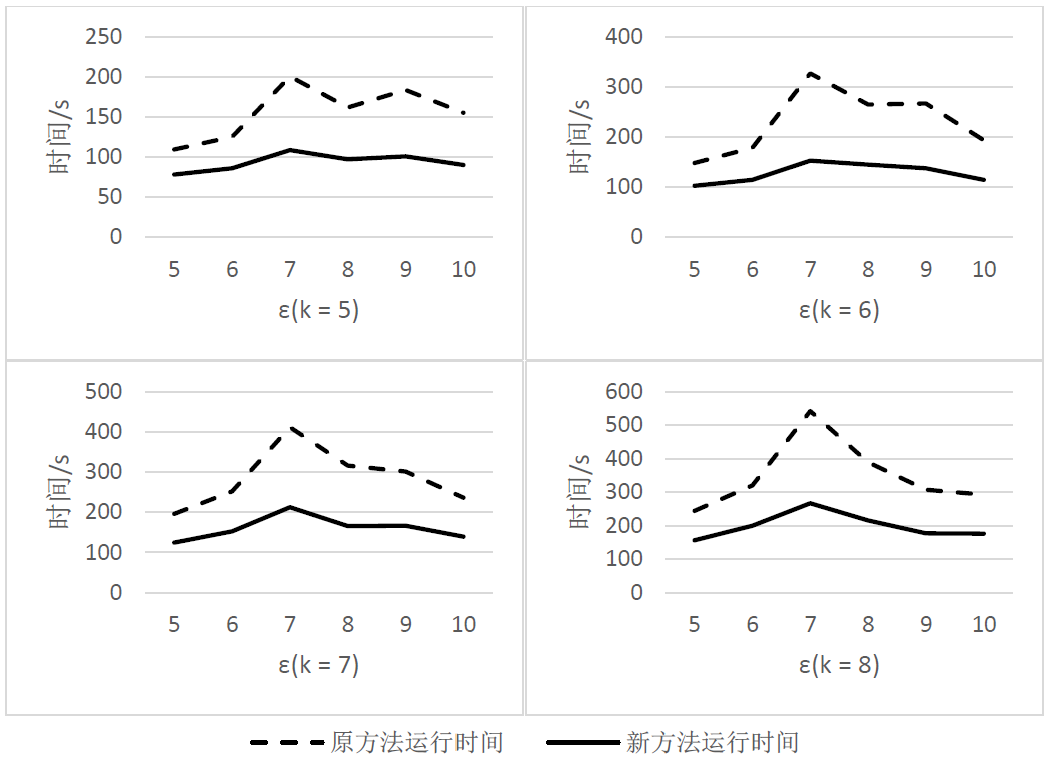
\includegraphics[width=0.55\textwidth]{figures/figure62x7Agas}
	\caption{模拟非周期时间采样的UCI气体数据上的运行时间,其中$k$是多项式次数,$\varepsilon$是拟合误差}\label{fig:fig627}
\end{figure}

\begin{figure}[htb]
	\centering
	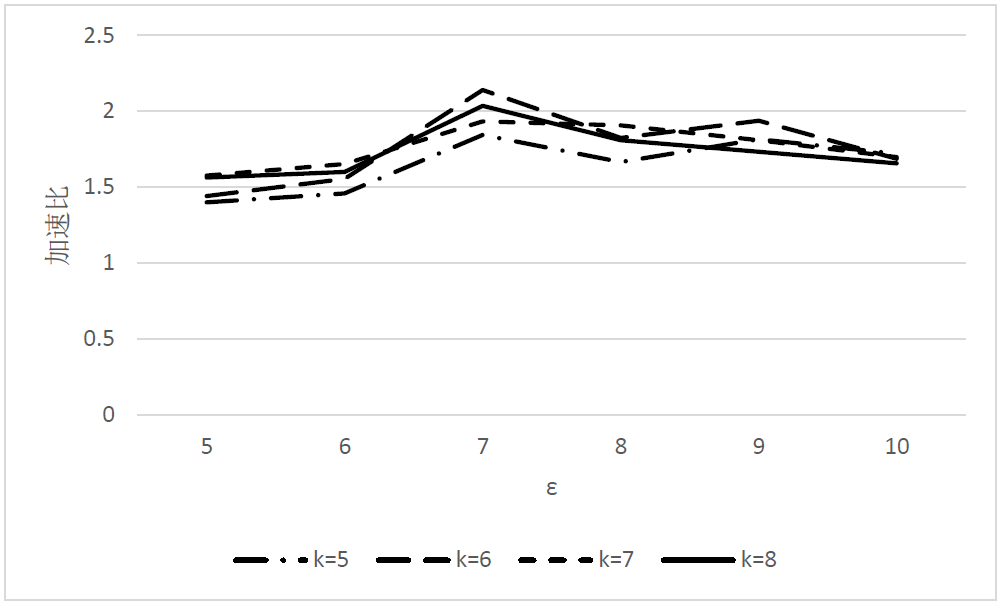
\includegraphics[width=0.55\textwidth]{figures/figure62x8Agas}
	\caption{模拟非周期时间采样的UCI气体数据上的加速比,其中$k$是多项式次数,$\varepsilon$是拟合误差}\label{fig:fig628}
\end{figure}
由图可知,其加速比在$1.4$x $\sim 2.2$x之间,最大可达$2.2$x,而且$k$越大,加速比越大,但其变化不大,甚至$k=8$时的加速比要整体小于$k=7$时的加速比。

在关于人体移动传感器数据集的实验中,因为采集时间间隔是不确定的,时刻序号是不确定的,而且相对来说某些时间间隔很大,即计算中$x_i$的值很大。所以,在计算过程中,会遇到矩阵$X$中的元素很大,以至于$X^TX$中的元素值很大,而对其求逆后,逆矩阵$(X^TX)^{-1}$中的元素值很小,接近于$0$,最终会出现逆矩阵为零矩阵的问题。为了解决这个问题,实验中对时刻序号进行处理,全部将其缩小十倍。最后,实验的运行时间结果如图\ref{fig:fig629}所示,其加速比如图\ref{fig:fig6210}所示。

\begin{figure}[htb]
	\centering
	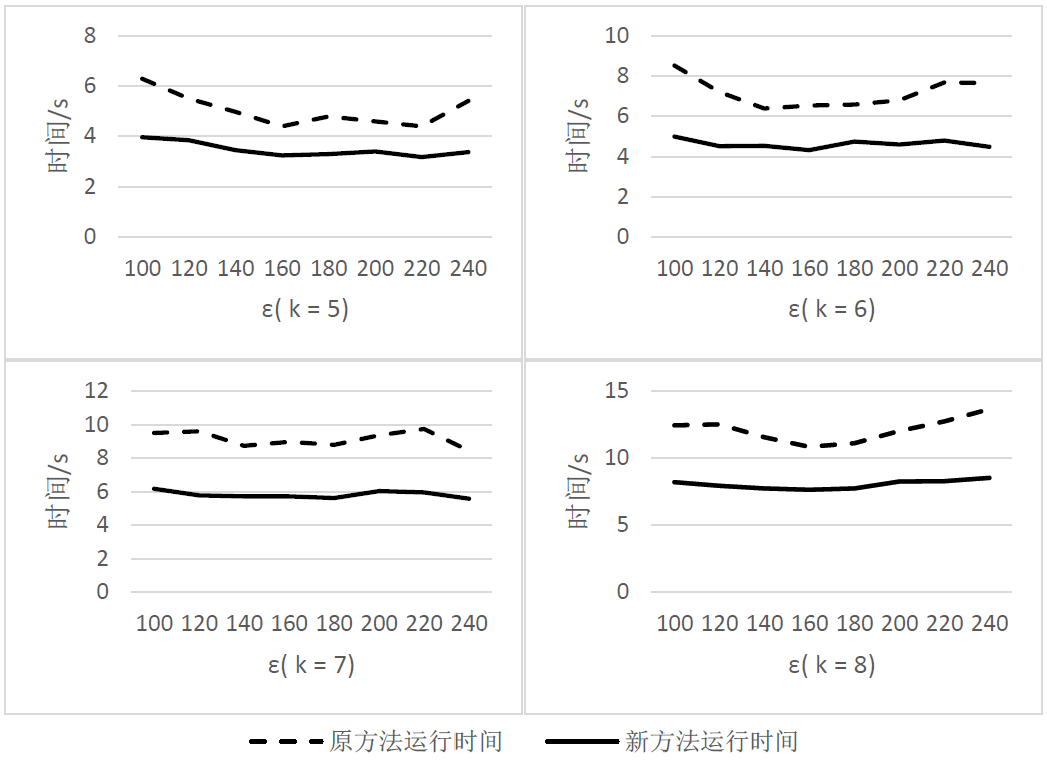
\includegraphics[width=0.55\textwidth]{figures/figure62x9Asen}
	\caption{非周期时间采样的UCI人体移动传感器数据上的运行时间,其中$k$是多项式次数,$\varepsilon$是拟合误差}\label{fig:fig629}
\end{figure}

\begin{figure}[htb]
	\centering
	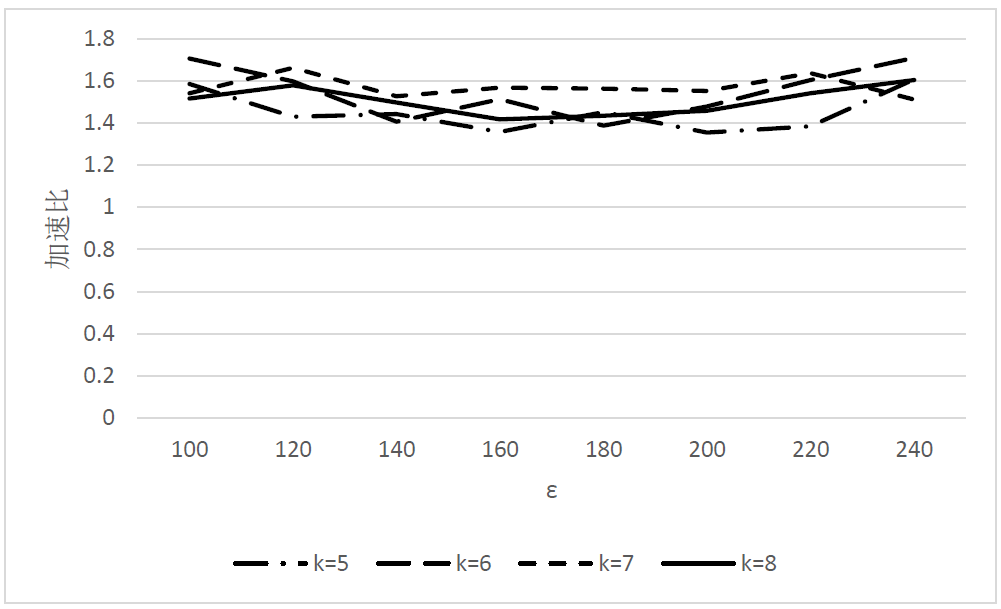
\includegraphics[width=0.55\textwidth]{figures/figure62x10Asen}
	\caption{非周期时间采样的UCI人体移动传感器数据集上的加速比,其中$k$是多项式次数,$\varepsilon$是拟合误差}\label{fig:fig6210}
\end{figure}

由图\ref{fig:fig629}可知,当多项式次数$k$不变时,运行时间基本不变,但是当$k$增大时,运行时间都会增大。由图\ref{fig:fig6210}可以看出,加速比基本在$1.4$x $\sim 1.7$x之间。从这两组实验数据可知,无论多项式次数$k$和拟合误差$\varepsilon$如何取值。在非周期时间采样时序数据上的加速方法可以达到加速效果。   

\section{本章小结} 
本章内容对本文提出的流式计算中的快速异常数据检测算法与数据压缩的加速方法进行了实验验证。在异常数据检测的实验中,分别选择了数据集,进行了增量的LOF算法与本文提出的加速算法的对比实验,实验结果发现,本算法可以较快地发现异常数据,而且使用内存容量更少,更能符合流式数据数据量大以及处理速度快的特点。  在对流式时序数据的压缩实验中,由实验结果可知,本文提出的方法,能够在周期时间采样的时序数据的压缩上达到很好的加速效果。而对于非周期时间采样的时序数据,虽然加速效果不如周期时间采样的时序数据,但是也可以达到$1.5$x倍的加速效果。                                    